\documentclass[serif, 12pt]{beamer}

\usepackage{graphicx} % Allows including images
\usepackage{booktabs} % Allows the use of \toprule, \midrule and \bottomrule in tables

\usepackage{color}

\usepackage{algorithm2e}
\usepackage{hyperref}

\newcommand*\mat[1]{ \begin{pmatrix} #1 \end{pmatrix}}
\newcommand*\arr[1]{ \begin{bmatrix} #1 \end{bmatrix}}
\newcommand*\V[1]{ \boldsymbol{#1}}

\newcommand*\D{\textcolor{violet}{D}}
\newcommand*\T{\textcolor{blue}{T}}

\setbeamertemplate{navigation symbols}{}%remove navigation symbols

\setbeamerfont{page number in head/foot}{size=\small}
\setbeamertemplate{footline}[frame number]

\title{Approximated PCA}

\author{Rodrigo Arias} % Your name
\date{\today} % Date, can be changed to a custom date

\begin{document}

\begin{frame}
	\titlepage
\end{frame}

%------------------------------------------------

\begin{frame}

\frametitle{PCA algorithm}

\begin{enumerate}
\item Take a dataset $X$ of $n$ variables.
\item Scale and center the variables.
\item From $X$ compute the $n\times n$ covariance matrix $S$.
\item \textbf{Compute the eigenvalues and eigenvectors of $S$.}
\item \textit{Optional: Ignore some eigenvectors.}
\item Generate a new basis from the selected eigenvectors.
\item Project $X$ into the new basis.
\end{enumerate}

\pause

Computing the eigenvectors is the principal step of PCA.

\end{frame}

%------------------------------------------------

\begin{frame}

\frametitle{Visual example}

The input dataset with $n=800$ variables and 1023 observations (columns),

$$ X=
	\mat{
		x_{1,1} & x_{1,2} 	& \dots & x_{1,1023}  \\
		x_{2,1} & x_{2,2}  	& \dots & x_{2,1023}  \\
		\vdots  & \vdots  	&       & \vdots      \\
		x_{800,1} & x_{800,2} & \dots & x_{800,1023} \\
	}
$$

Each pixel $x_{i,j}$ is a value in $[0, 255]$ of the gray level in the image.  

\end{frame}

%------------------------------------------------

\begin{frame}

\frametitle{Visual example}

The input dataset with $n=800$ variables and 1023 observations (columns), $X =$

\begin{center}
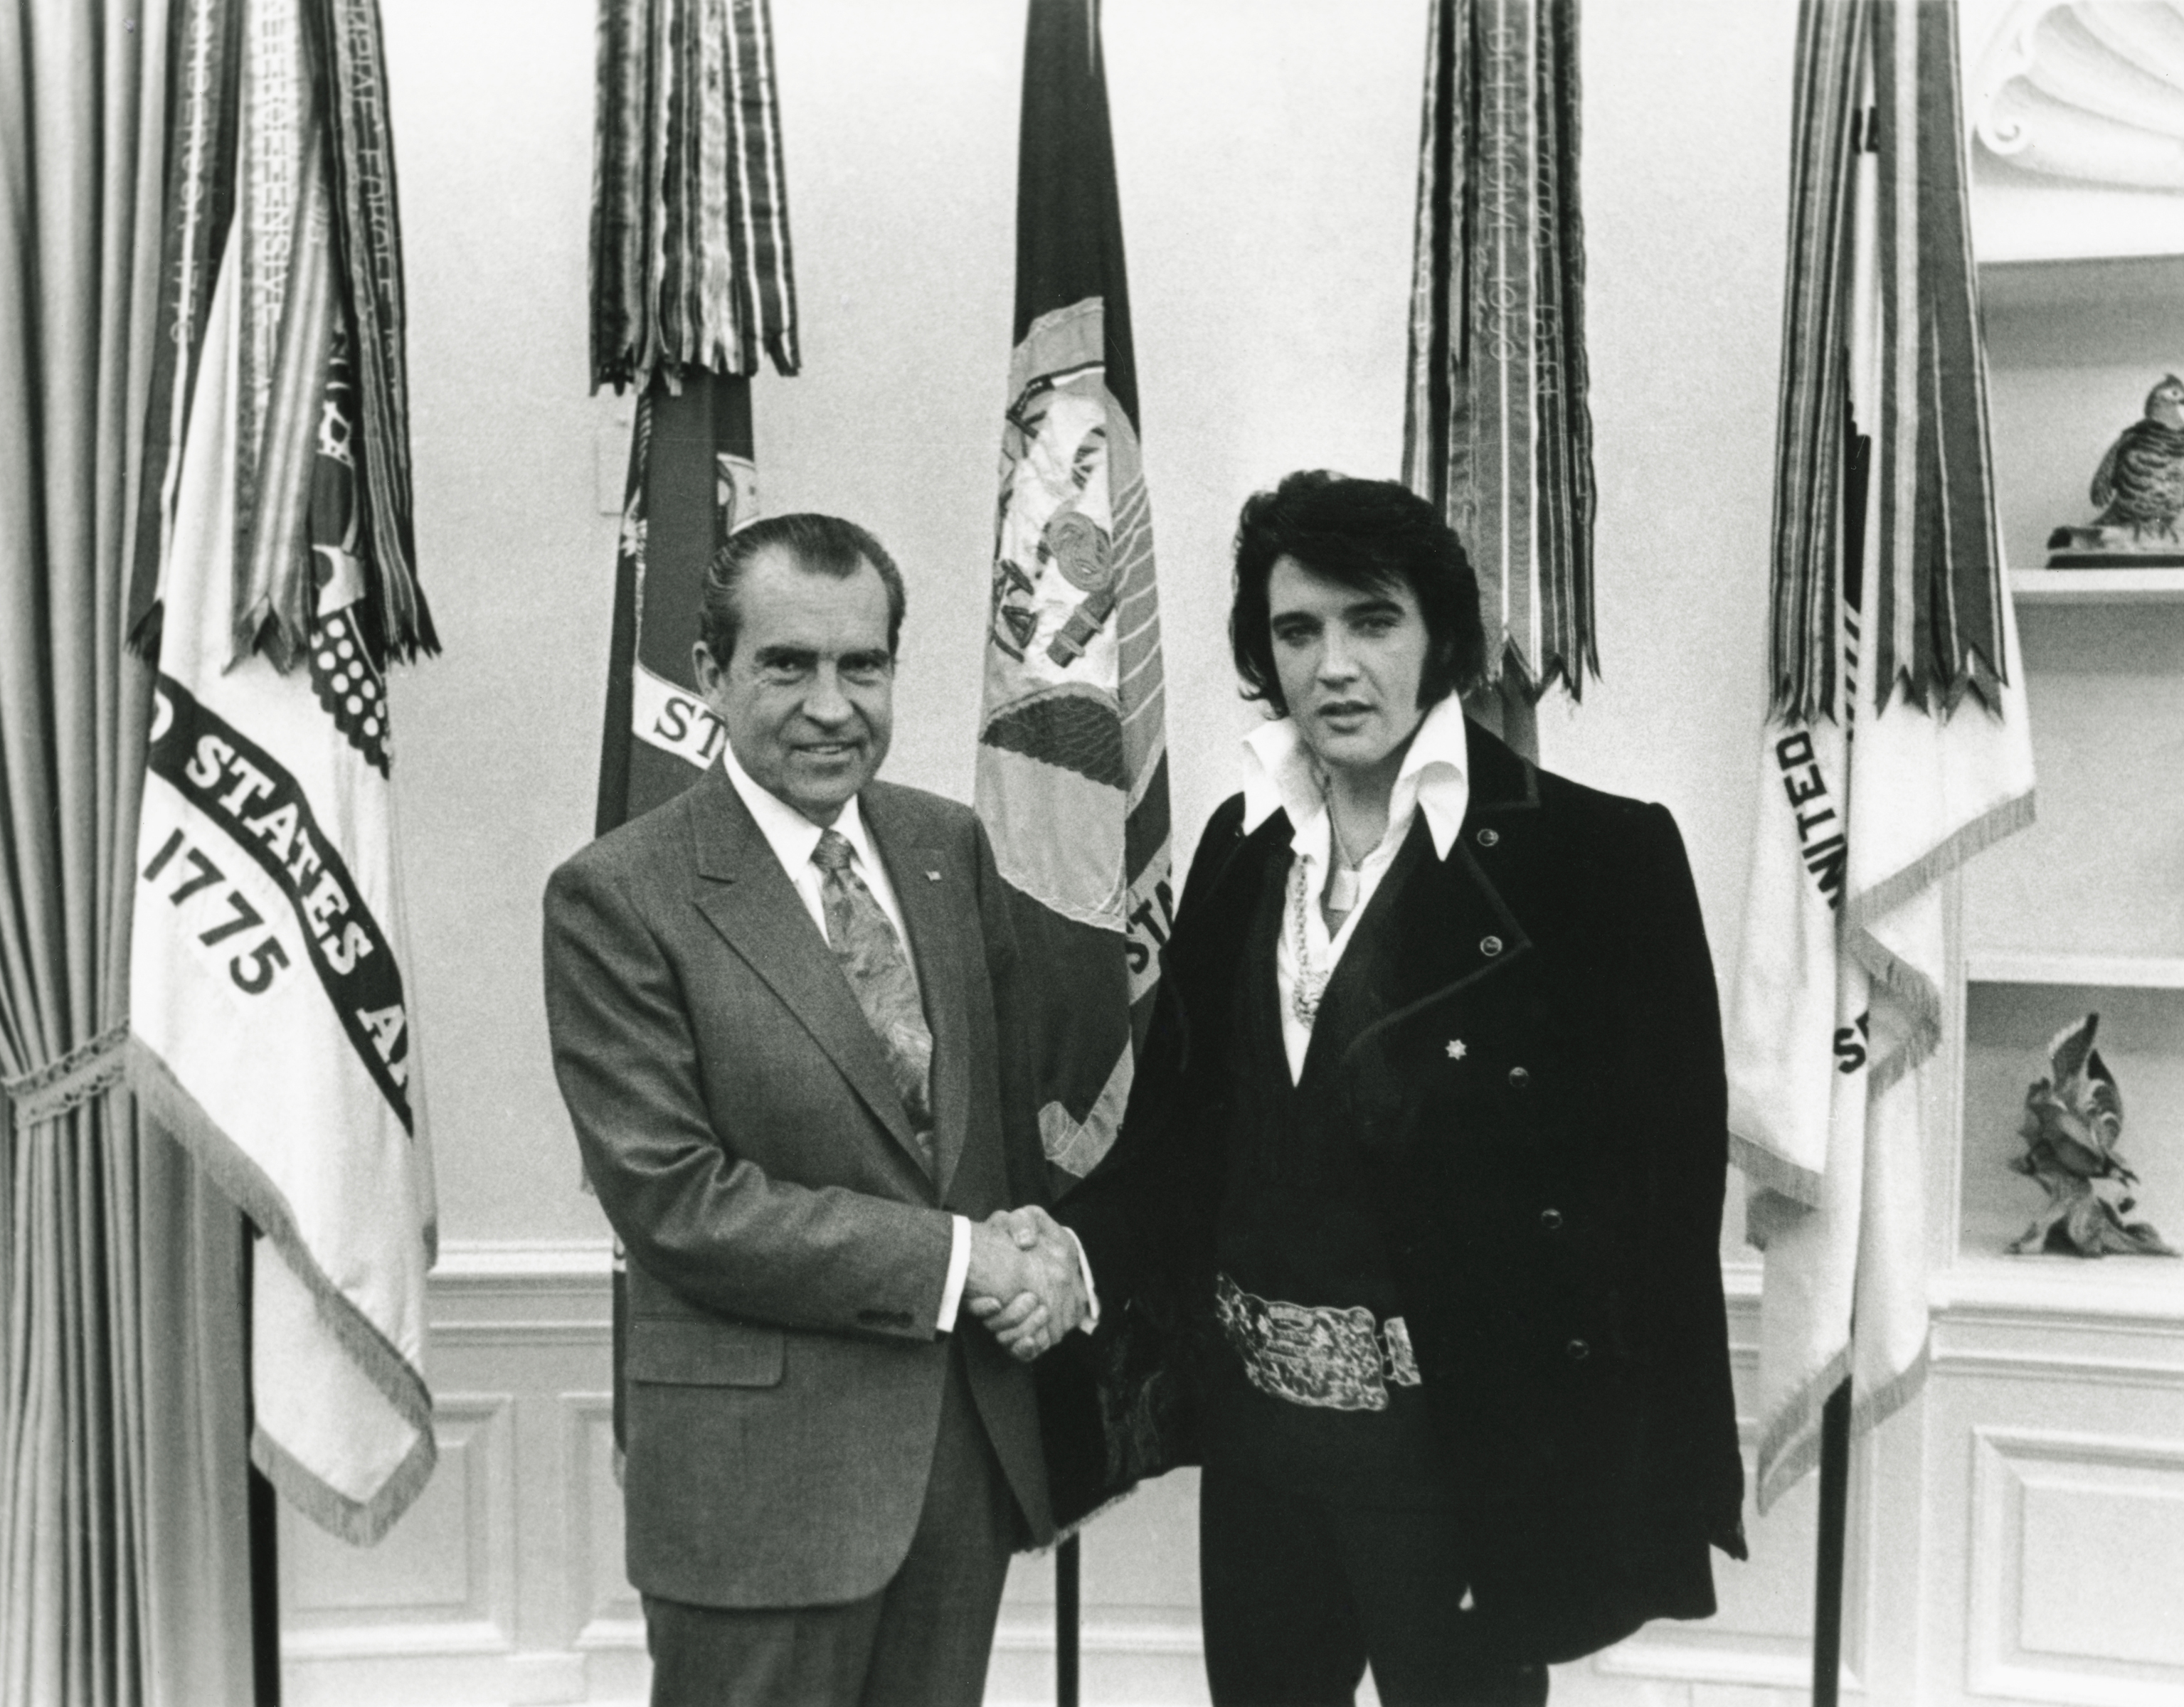
\includegraphics[scale=0.2]{input}
\end{center}

Each pixel $x_{i,j}$ is a value in $[0, 255]$ of the gray level in the image.  

\end{frame}

%------------------------------------------------

\begin{frame}

\frametitle{Visual example}
Keep 800 eigenvectors. Output:

\begin{center}
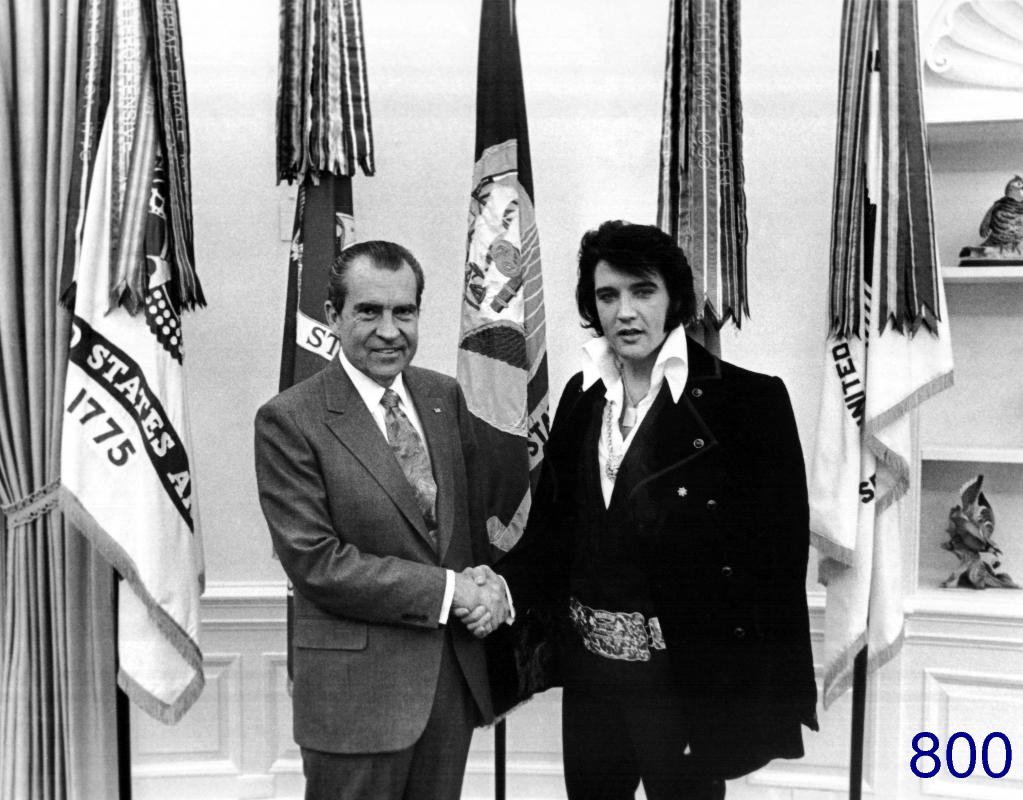
\includegraphics[width=\textheight]{out-800}
\end{center}

\end{frame}


%------------------------------------------------

\begin{frame}

\frametitle{Visual example}
Keep 200 eigenvectors. Output:

\begin{center}
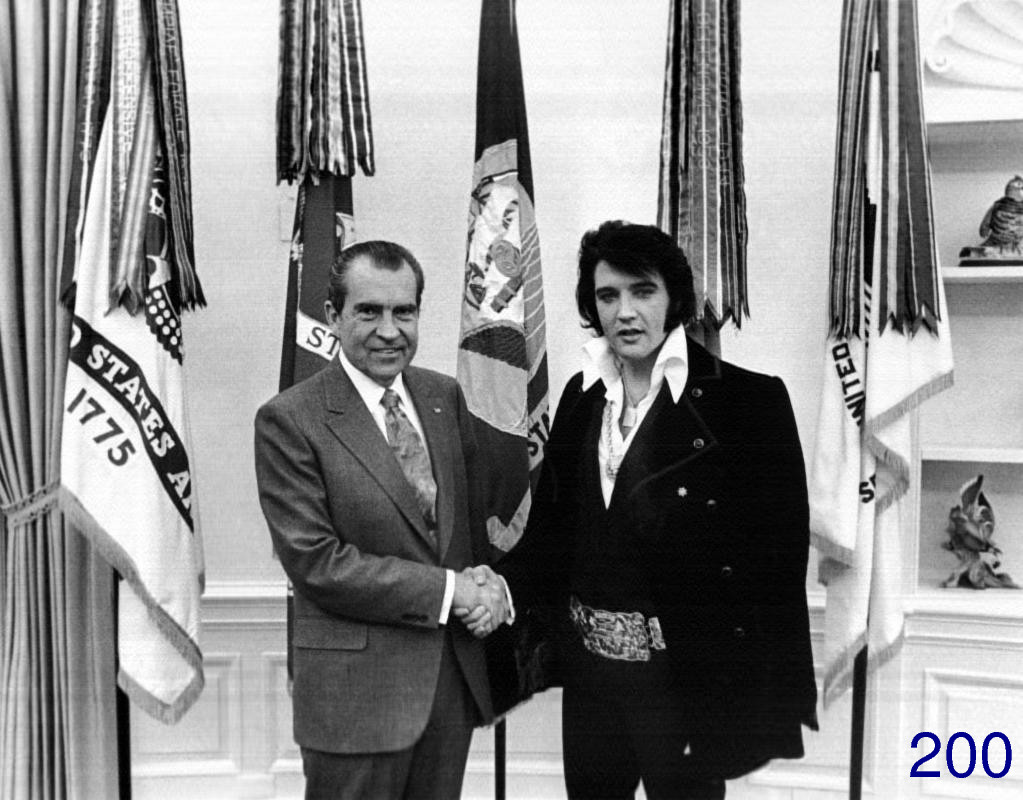
\includegraphics[width=\textheight]{out-200}
\end{center}

\end{frame}

%------------------------------------------------

\begin{frame}

\frametitle{Visual example}
Keep 100 eigenvectors. Output:

\begin{center}
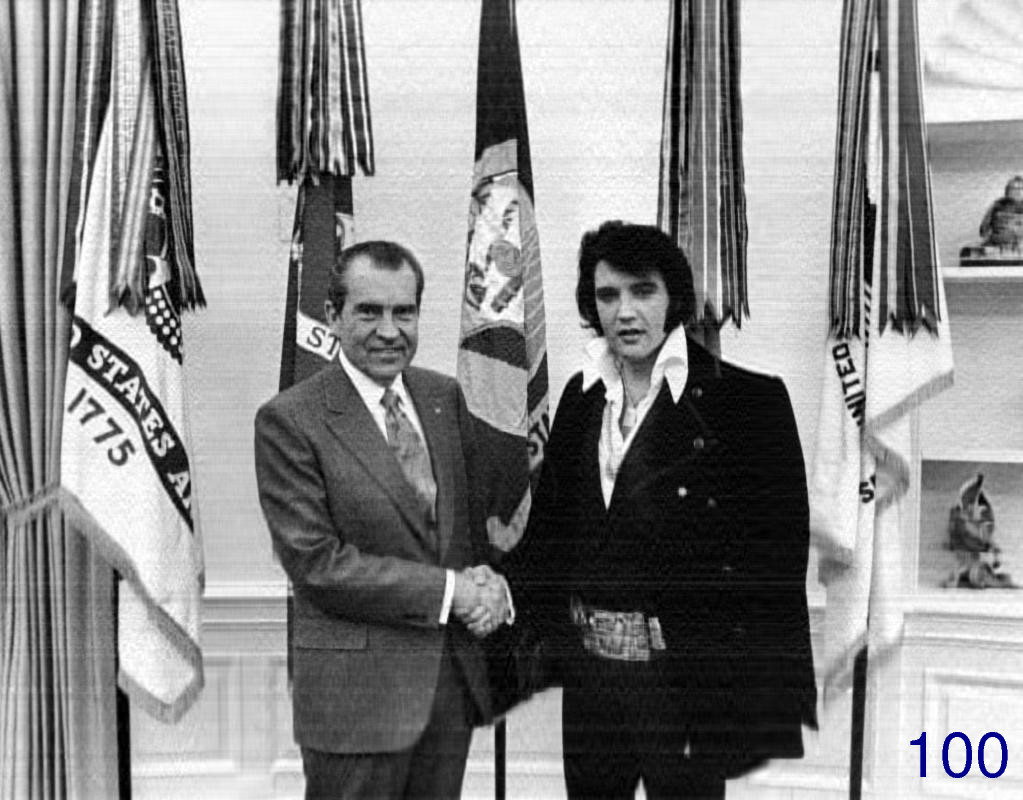
\includegraphics[width=\textheight]{out-100}
\end{center}

\end{frame}

%------------------------------------------------

\begin{frame}

\frametitle{Visual example}
Keep 40 eigenvectors. Output:

\begin{center}
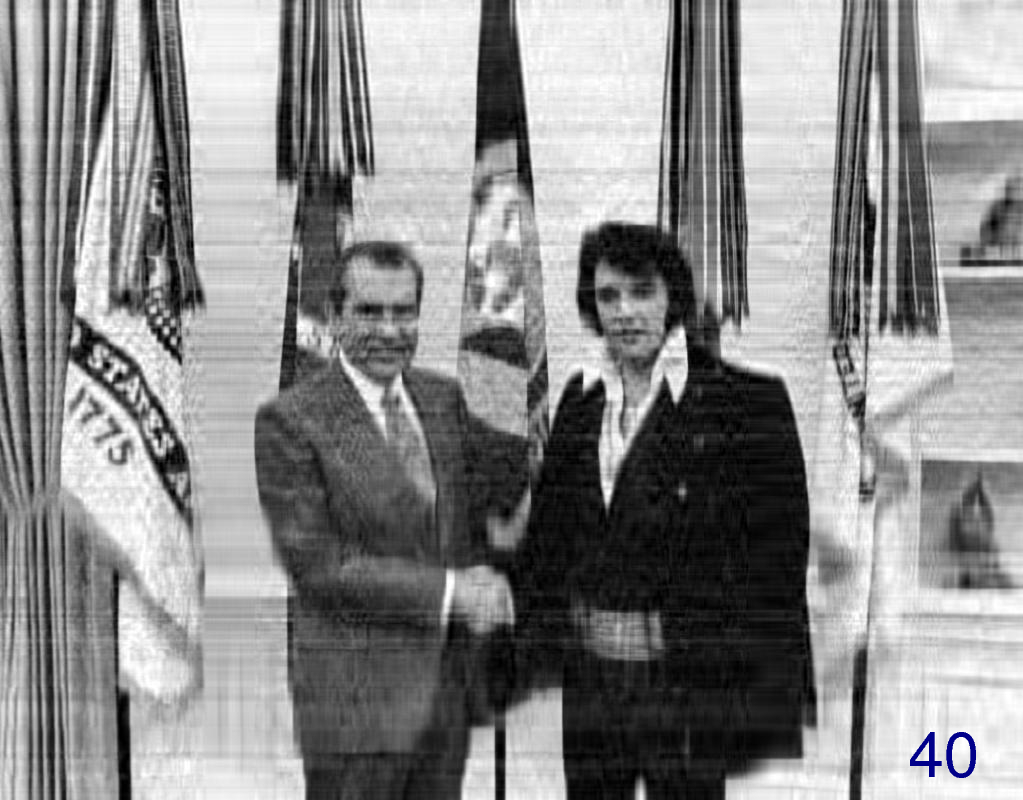
\includegraphics[width=\textheight]{out-40}
\end{center}

\end{frame}

%------------------------------------------------

\begin{frame}

\frametitle{Computing eigenvalues and eigenvectors}

\begin{enumerate}
\item Take the $n\times n$ target matrix $A = S$.
\item Compute a \textcolor{blue}{tridiagonal} matrix $\T$: $A = P \T P^T$.
\item From $\T$ compute a \textcolor{violet}{diagonal} matrix $\D$: $\T = Q \D 
Q^T$.
\item The eigenvalues of $A$ are in the diagonal of $\D$.
\item Compute the eigenvectors from $\D$.
\end{enumerate}

\pause

Computing a tridiagonal matrix is called \textbf{tridiagonalization}. For the 
diagonal, \textbf{diagonalization}. Several algorithms exists for both steps.

\end{frame}


%------------------------------------------------

\begin{frame}
%
\frametitle{Tridiagonalization}
%
These algorithms transform a \textbf{symmetric} matrix $A$ into a new pair of 
matrices $P$ and $\T$ such that $P$ is orthogonal, $\T$ is tridiagonal, and $A = 
P \T P^T$
%
$$
	\mat{
		a_{11} & a_{12} & a_{13} & a_{14} \\
		a_{21} & a_{22} & a_{23} & a_{24} \\
		a_{31} & a_{32} & a_{33} & a_{34} \\
		a_{41} & a_{42} & a_{43} & a_{44} \\
	} =
	P
	\textcolor{blue}{
	\mat{
		t_{11} & t_{12} &        &        \\
		t_{21} & t_{22} & t_{23} &        \\
		       & t_{32} & t_{33} & t_{34} \\
		       &        & t_{43} & t_{44} \\
	}}
	P^T
$$
%
\end{frame}

%------------------------------------------------

\begin{frame}
%
\frametitle{Tridiagonalization}
%
\begin{center}
\begin{tabular}{c c c c}
	\toprule
	Algorithm 		& Complexity  & Iterative & Stability\\
	\midrule
	Householder		& $O(4n^3/3)$ & No        & Great\\
	Givens				& $O(kn^3)$   & No        & Good \\
	Lanczos				& $O(kpn^2)$  & Yes       & Bad \\
	Others				&             &          \\
	\bottomrule
\end{tabular}
\end{center}
Where $n \times n$ is the dimension of the matrix $A$, $k$ is some constant, and 
$p$ the number of iterations.
\end{frame}

%------------------------------------------------

\begin{frame}
%
\frametitle{Diagonalization}
%
These algorithms take a \textbf{tridiagonal} matrix $\T$ into a new pair of 
matrices $Q$ and $\D$ such that $Q$ is orthogonal, $\D$ is diagonal, and $\T = Q 
\D Q^T$
%
$$
	\textcolor{blue}{
	\mat{
		t_{11} & t_{12} &        &        \\
		t_{21} & t_{22} & t_{23} &        \\
		       & t_{32} & t_{33} & t_{34} \\
		       &        & t_{43} & t_{44} \\
	}}=
	Q
	\textcolor{violet}{
	\mat{
		d_{11} &        &        &        \\
		       & d_{22} &        &        \\
		       &        & d_{33} &        \\
		       &        &        & d_{44} \\
	}}
	Q^T
$$
%
The matrix $\D$ contains the \textbf{eigenvalues} in the diagonal.
\end{frame}

%------------------------------------------------

\begin{frame}
%
\frametitle{Diagonalization}
%
\begin{center}
\begin{tabular}{c c c c}
	\toprule
	Algorithm							& Complexity  & Convergence	\\
	\midrule
	QR                  & $O(6n^3)$ 	& Cubic 			\\
	Divide and conquer  & $O(8n^3/3)$ & Quadratic 	\\
	Jacobi              & $O(n^3)$    & Quadratic 	\\
	Power iteration			& $O(n^3)$    & Linear 			\\
	Inverse iteration	  & $O(n^3)$    & Linear 			\\
	Others							&             &          		\\
	\bottomrule
\end{tabular}
\end{center}
%
All these algorithms are iterative and $n \times n$ is the dimension of the 
matrix $A$.
\end{frame}

%------------------------------------------------

\begin{frame}
%
\frametitle{The selected method}
%
\centering
Householder + QR
\end{frame}

%------------------------------------------------

\begin{frame}
%
\frametitle{Approximated computing}
%
Maximize an utility function, based on your preferences:
$$ \max \; u(E, T, n, \epsilon, C, \ldots) $$

\begin{center}
\begin{tabular}{c l}
	$E$ & Energy consumption \\
	$T$ & Time taken\\
	$n$ & Problem size \\
	$\epsilon$ & Error in the result \\
	C &  Economical cost \\
	$u()$ & Utility function \\
\end{tabular}
\end{center}

\end{frame}

%------------------------------------------------

\begin{frame}
%
\frametitle{Techniques: Deterministic}
%
\begin{itemize}
\item \textbf{Bit-Width Reduction}
\item Float-to-Fixed Conversion
\item Fuzzy Memoization
\item Hierarchical FPU
\item Load Value Approximation
\item Lossy Compression and Data
\item Packing
\item Precision Scaling (ALU)
\item Reduced-Precision FPU
\item Underdesigned Multiplier
\item ...
\end{itemize}

\pause

Begin with bit-width reduction
\end{frame}

%------------------------------------------------

\begin{frame}
%
\frametitle{Bit-width reduction in Householder}
%
\begin{itemize}
\item The Householder algorithm performs $n-2$ steps.
\item In each step, a matrix multiplication is done.
\item With less precision, the error in the final result can grow.
\item Analyze how the error changes in Householder.
\end{itemize}

\end{frame}

%------------------------------------------------

\begin{frame}
%
\frametitle{Bit-width reduction in Householder}
%
\begin{itemize}
\item Some theoretical bounds can be used to check the experimental error
\item Design a emulator with an ALU of $b$ bit-width
\item Test the algorithm in the emulator with different $b$, and check the 
error.
\end{itemize}

\end{frame}

\end{document}
